\section{Problem Setup}
\label{sec:setup}

This section formalises the TS DA setting and surveys the landscape of existing generative DA methods.
Section~\ref{sec:setup:ts-da} fixes notation. The remainder
positions ASCENSION in the broader literature.

% -----------------------------------------------------------------
% ADDED FOR TMLR (structural — TMLR DA paper convention folds
% related work into a Problem Setup section, cf.~Mai \& Lin
% TMLR 2024, \S2).
% -----------------------------------------------------------------
\subsection{Time-series data augmentation}
\label{sec:setup:ts-da}
 DA aims to expand the training set with synthetic samples to increase the generalisation ability of the trained model \citep{shorten2019survey}, primarily by
  reducing overfitting, which we measure operationally in our setting as performance on the test set. Formally, let $\mathcal{D} = \{(x_i, y_i)\}_{i=1}^{N}$ be a labelled  
  TS dataset with $x_i \in \mathbb{R}^{T}$ a univariate
  series of length $T$ and $y_i \in \{1, \ldots, Y\}$ a class label.  
  A DA method produces an auxiliary set  
  $\mathcal{D}' = \{(x'_j, y'_j)\}_{j=1}^{M}$. The objective
  is for a classifier trained on $\mathcal{D} \cup \mathcal{D}'$ to 
  reach higher test-set accuracy than one trained on $\mathcal{D}$
  alone (or at least not lower). 
  
  One of the main challenges for DA in TSC is not that no
  method helps on some datasets, but that no single
  method helps reliably across the heterogeneous domains  
  encountered in practice (ECG, accelerometer, image-derived,
  spectral, motion, power). Empirical studies 
  \citep{iwana2021empirical, iglesias2023data} have
  documented this inconsistency: DA methods that win on one
  dataset (resp. domain) degrade accuracy on the next. As a  
  result, practitioners face the real overhead of testing several 
  DA methods on each new dataset to find one that does not hurt, a
  cost that scales with the number of methods available and grows 
  as the literature expands. ASCENSION is designed to reduce that 
  cost. Therefore, our evaluation jointly targets: (i) the average gain, as the method should improve mean test-set accuracy across a large benchmark, (ii) the gain consistency, so that it can be adopted without a per-dataset method-selection loop.  

  We report both metrics in Section~\ref{sec:results:main}. 
  

\subsection{Related work}
\label{sec:setup:gen-da}
\begin{figure*}[t]
  \centering
  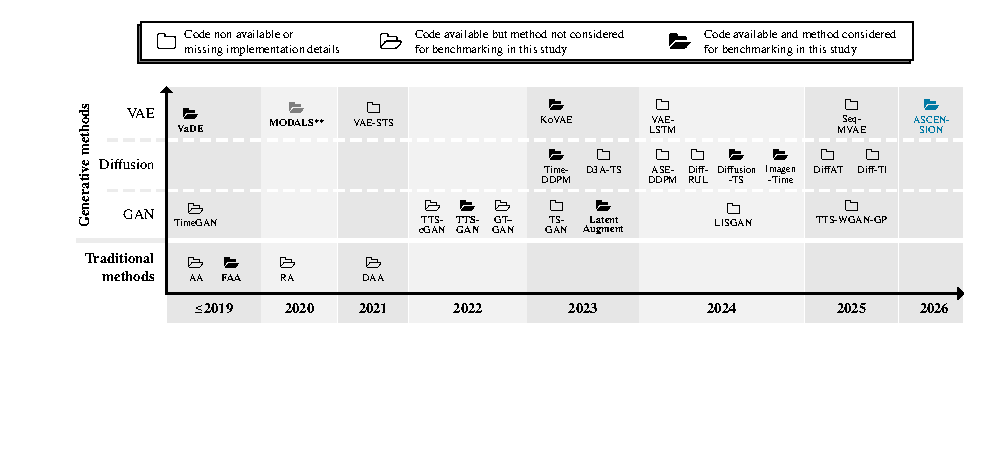
\includegraphics[trim=1cm 2.25cm .1cm 0cm,clip,width=\textwidth]{images/SoTa_evolution_DA}
\caption{Overview of state-of-the-art DA methods for TS (traditional vs. generative). \textbf{MODALS**}: Although the code was released 6~years ago, it is now non-functional; the authors confirmed it cannot be restored without major re-coding. We therefore compare ASCENSION and MODALS on the HAR dataset used in \cite{cheung2020modals}.}
  \label{fig:SoTa}
\end{figure*}

% REVISED FOR TMLR (rebuttal Q1): survey condensed to its positioning
% essentials, the complete discussion moves verbatim to
% Appendix~\ref{app:related-extended}.
TS DA methods can be classified as traditional or
generative according to \citep{iglesias2023data, iwana2021empirical}
and summarised in Figure~\ref{fig:SoTa}.

\paragraph{Traditional DA methods}
Traditional methods such as window slicing, jittering, and scaling
apply predefined transformations adapted from computer vision, and
automated successors such as \textbf{AutoAugment (AA)}
\citep{cubuk2019autoaugment}, \textbf{Fast AutoAugment (FAA)}
\citep{lim2019fast}, \textbf{RandAugment} \citep{cubuk2020randaugment},
\textbf{Deep AutoAugment} \citep{zheng_deep_2022}, and \textbf{Trivial
Augment} \citep{muller2021trivialaugment} automate the search for
transformation policies. Because the transformations remain
predefined, they can disrupt the semantic integrity of TS data and
struggle to preserve intra-class consistency. For instance, reversing
the time axis of an electrocardiogram sequence can render it
meaningless.

\paragraph{Generative DA methods}
Generative models, such as Generative Adversarial Networks (GANs)
\citep{goodfellow2020generative}, diffusion models
\citep{yang2023diffusion}, and VAEs \citep{kingma2013auto}, learn a
probabilistic representation of the data distribution and can
generate TS that retain temporal dependencies and class-specific
characteristics \citep{fu2020data}. GAN-based DA methods, from TimeGAN
\citep{zhang2022data} and TS-GAN \citep{yang2023ts} to GT-GAN
\citep{jeon2022gt}, TTS-GAN and its conditional variant
\citep{li2022tts, li2022ttsc}, LatentAugment
\citep{tronchin2023latentaugment}, LISGAN \citep{seon2024least},
and TTS-WGAN-GP \citep{mousavi2025transformer}, generate realistic
sequences but are notoriously unstable to train and prone to mode
collapse \citep{lei2019mode}.

Diffusion-based DA
methods, from SE-DDPM \citep{liu2024adaptive} and DiffRUL
\citep{wang2024diffrul} to D3A-TS \citep{solis2023}, Time-DDPM
\citep{dai2023timeddpm}, Diffusion-TS \citep{yuandiffusion},
ImagenTime \citep{naiman2024utilizing}, DiffAT \citep{yu2025diffat},
and Diff-TI \citep{zhang2025time}, produce stable outputs but still
face challenges with long-range dependencies, error accumulation, and
slow inference \citep{feng2024latent}.
% ADDED FOR TMLR (AE request: small-sample generative benchmark)
Under data scarcity these models degrade further: in the first
large-scale study of generative TS models in this regime,
\citet{gonen2025time} show that generation quality collapses as
training sets shrink, and mitigate this by pretraining a unified
diffusion model on a large collection of datasets before
fine-tuning it on the target one.

VAEs allow explicit control over the
diversity of generated samples through manipulation of the latent
space, are less prone to collapse than GANs, and are less
computationally expensive than both alternatives
\citep{thanh2020catastrophic}, which motivates our choice of this
family. Within VAE-based DA, \textbf{VaDE} \citep{jiang2016variational} and
\textbf{GMVAE} \citep{dilokthanakul2017gmvae} structure the latent
space with a Gaussian Mixture Model (GMM). In both cases, the mixture
is an unsupervised inductive bias: it is part of the generative model
and appears in the evidence lower bound (ELBO), and neither method
provides a mechanism to control the extent of generation beyond the
learned distribution. \textbf{MODALS} \citep{cheung2020modals} was
the first study to explore class boundary expansion during synthetic
data generation, though it lacks a mechanism to control the extent of
this expansion.
% ADDED FOR TMLR (AE request: discuss KoVAE as the VAE generation
% baseline)
\textbf{KoVAE} \citep{naiman2023generative} places a linear
Koopman prior on the latent dynamics, which yields an interpretable
model of both regular and irregular TS and high-fidelity samples
from the learned distribution. Like VaDE and GMVAE, however, it
provides no mechanism to generate beyond that distribution: its
samples remain confined to the density it has learned. We analyse
the empirical consequence of this difference in
Section~\ref{sec:results:main}.
% ADDED FOR TMLR (AE request: covariance-based latent expansion
% precedents)
Expanding class representations through their covariance has
precedents outside TS classification, in image classification
\citep{wang2019implicit}, speaker recognition \citep{wang2020data},
and agronomic data \citep{lan2025cotton}, discussed in
Appendix~\ref{app:related-extended}. Other VAE variants target
specific priors or modalities \citep{goubeaud2021using, dang2024vae,
bogojeski2025data}. However, none of these approaches explore a
progressive, tunable expansion of class representations in the
latent space, as proposed in ASCENSION. The complete discussion is provided in
Appendix~\ref{app:related-extended}.
